\chapter{Revisão Bibliográfica}

No presente capítulo, são apresentados conceitos básico para a compreensão do presente trabalho. Nessa etapa, busca-se através da revisão de trabalhos já elucidados a contextualização do projeto proposto.

\section{CONCEITOS BÁSICOS}

%Esta seção desenvolverá conceitos fundamentais para a compreensão da problemática resolvida com o sistema proposto. O objeto de estudo emerge à evidência quando observados dois atores opostos: a complexidade do sistema e sua robustez. Estes são primeiramente compreendidos pela natureza de um sistema embarcado.

Esta seção explanará conceitos bás

\subsection{SITEMAS DE CONTROLE}
 
\subsection{CONTROLADORES}

\subsection{SINTONIA DE CONTROLADORES}

\subsection{CONTROLADORES PID}

\begin{figure}[htb]
	\caption{Representação Clássica do Modelo de Controlador PID}
	\begin{center}
	    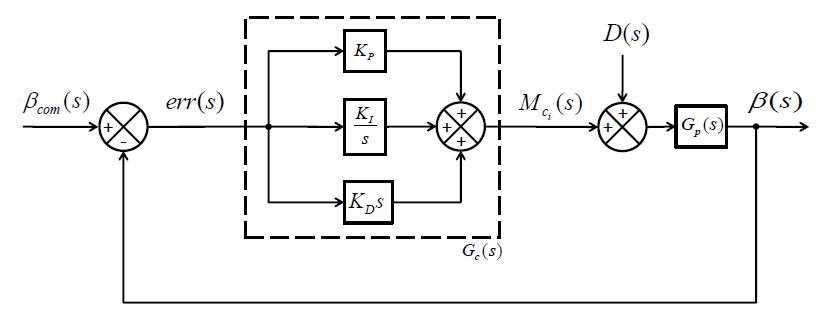
\includegraphics[scale=0.75]{img/pid_controller.PNG}
	\end{center}
	\fonte{Adaptado de \citeonline{Verma2018}.} 
\end{figure}


\begin{figure}[htb]
	\caption{Representação do Modelo de Controlador PID com distúrbios}
	\begin{center}
	    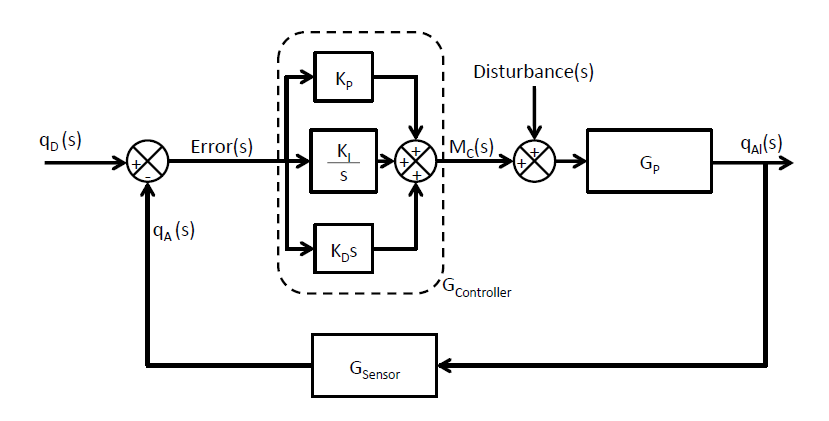
\includegraphics[scale=0.75]{img/pid_disturbe}
	\end{center}
	\fonte{Adaptado de \citeonline{Verma2018}.} 
\end{figure}


\subsection{INTELIGÊNCIA ARTIFICIAL}

\subsection{SISTEMA EMBARCADO}

\section{ESTADO DA ARTE}

\subsection{SISTEMAS INTELIGENTES DE SINTONIA AUTOMÁTICA}